\documentclass[a4paper,12pt]{article}
%%%%%%%%%%%%%%%%%%%%%%%%%%%%%%%%%%%%%%%%%%%%%%%%%%%%%%%%%%%%%%%%%%%%%%%%%%%%%%%%%%%%%%%%%%%%%%%%%%%%%%%%%%%%%%%%%%%%%%%%%%%%%%%%%%%%%%%%%%%%%%%%%%%%%%%%%%%%%%%%%%%%%%%%%%%%%%%%%%%%%%%%%%%%%%%%%%%%%%%%%%%%%%%%%%%%%%%%%%%%%%%%%%%%%%%%%%%%%%%%%%%%%%%%%%%%
\usepackage{eurosym}
\usepackage{vmargin}
\usepackage{amsmath}
\usepackage{graphics}
\usepackage{epsfig}
\usepackage{subfigure}
\usepackage{fancyhdr}
%\usepackage{listings}
\usepackage{framed}
\usepackage{graphicx}

\setcounter{MaxMatrixCols}{10}
%TCIDATA{OutputFilter=LATEX.DLL}
%TCIDATA{Version=5.00.0.2570}
%TCIDATA{<META NAME="SaveForMode" CONTENT="1">}
%TCIDATA{LastRevised=Wednesday, February 23, 2011 13:24:34}
%TCIDATA{<META NAME="GraphicsSave" CONTENT="32">}
%TCIDATA{Language=American English}

\pagestyle{fancy}
\setmarginsrb{20mm}{0mm}{20mm}{25mm}{12mm}{11mm}{0mm}{11mm}
\lhead{Dublin \texttt{R}} \rhead{10 April 2013}
\chead{Introduction to \texttt{R} (Module A)}
%\input{tcilatex}


\begin{document}

\tableofcontents
\newpage

\subsection{Pseudo-R Squared}
Cox  and Snell R Square and Nagelkerke R Square - These are pseudo R-squares.  Logistic regression does not have an equivalent to the R-squared that is found in OLS regression; however, many people have tried to come up with one.  

There are a wide variety of pseudo-R-square statistics (these are only two of them).  Because this statistic does not mean what R-squared means in OLS regression (the proportion of variance explained by the predictors), we suggest interpreting this statistic with great caution.
%---------------------------------------------------------- %
\newpage

\subsection{Psuedo R Squared Values}
%http://statistics.ats.ucla.edu/stat/mult_pkg/faq/general/Psuedo_RSquareds.htm

Cox \& Snell R Square and Nagelkerke R Square are two measures from the \textbf{pseudo R-squares} family of measures.


There are a wide variety of pseudo-R-square statistics (these are only two of them).  Because this statistic does not mean what R-squared means in OLS regression (the proportion of variance explained by the predictors), we suggest interpreting this statistic with great caution.


\subsection{Pseudo R-squares}
Cox \& Snell R Square and Nagelkerke R Square are two measures from the \textbf{pseudo R-squares} family of measures.

Logistic regression does not have an equivalent to the R-squared that is found in OLS regression; however, many researcehrs have tried to come up with one.  There are a wide variety of pseudo-R-square statistics.  

Because this statistic does not mean what R-squared means in OLS regression (the proportion of variance explained by the predictors), we suggest interpreting this statistic with great caution.

\subsubsection{Cox \& Snell R Square}
Cox and Snell's R-Square is an attempt to imitate the interpretation of multiple R-Square based on the likelihood, but its maximum can be (and usually is) less than 1.0, making it difficult to interpret. It is part of SPSS output.

\subsubsection{Nagelkerke's R-Square}
Nagelkerke's R-Square is a further modification of the Cox and Snell coefficient to assure that it can vary from 0 to 1. Nagelkerke's R-Square will normally be higher than the Cox and Snell measure. It is part of SPSS output and is the most-reported of the R-squared estimates.



\section{R Squared Diagnostics}
\begin{itemize}
	\item In order to understand how much variation in the dependent variable can be explained by the model (the equivalent of $R^2$ in multiple regression), you should consult \textbf{\textit{Model Summary}} statistics.
	
	\item 
	Logistic regression does not have an equivalent to the R-squared that is found in OLS regression; however, many researchers have tried to come up with one. 
	
	
	\item The SPSS output table below contains the \textit{Cox \& Snell R Square} and \textit{Nagelkerke R Square }values, which are both methods of calculating the explained variation. These values are sometimes referred to as pseudo $R^2$ values (and will have lower values than in multiple regression).
	\item  However, they are interpreted in the same manner, but with more caution. Therefore, the explained variation in the dependent variable based on our model ranges from 24.0\% to 33.0\%, depending on whether you reference the Cox \& Snell $R^2$ or Nagelkerke $R^2$ methods, respectively. 
	
	\item Nagelkerke $R^2$ is a modification of Cox \& Snell $R^2$, the latter of which cannot achieve a value of 1. For this reason, it is preferable to report the Nagelkerke $R^2$ value.
\end{itemize}

\begin{figure}[h!]
	\centering
	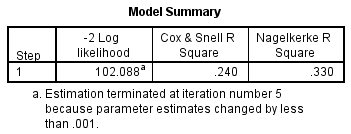
\includegraphics[width=0.9\linewidth]{images/BLogReg-Rsq}
	\caption{SPSS output}
	\label{fig:BLogReg-Rsq}
\end{figure}
\begin{itemize}
	\item Although there is no close analogous statistic in logistic regression to
	the coefficient of determination $R^2$ the Model Summary Table provides some approximations. Cox and Snell�s R-Square attempts to imitate multiple R-Square based on �likelihood�, but its maximum can be (and usually is) less than 1.0, making it difficult to interpret. 
	\item Here it is indicating that 55.2\% of the variation in the DV is explained by the
	logistic model. 
	\item Logistic regression does not have an equivalent to the R-squared that is found in OLS regression; however, many people have tried to come up with one.  
	Cox  and Snell R Square and Nagelkerke R Square - These are pseudo R-squares. 
	\item 	Nagelkerke's R-Square is a further modification of the Cox and Snell coefficient to assure that it can vary from 0 to 1. Nagelkerke's R-Square will normally be higher than the Cox and Snell measure. It is part of SPSS output and is the most-reported of the R-squared estimates.
	
	\item The Nagelkerke modification that does range from 0 to 1 is a more reliable
	measure of the relationship. Nagelkerke�s $R^2$ will normally be higher than the Cox and Snell measure.
	
	
	
	\item \textbf{Cox and Snell's R-Square} is an attempt to imitate the interpretation of multiple R-Square based on the likelihood, but its maximum can be (and usually is) less than 1.0, making it difficult to interpret. It is part of SPSS output.
\end{itemize}
%==============================================================%

\subsubsection{Nagelkerke's R-Square}
\begin{itemize}
	\item  Nagelkerke�s $R^2$ is part of SPSS output in the �Model Summary� table and is the most-reported of the R-squared estimates. 
	\item In our case it is 0.737, indicating a moderately strong relationship of 73.7\% between the predictors and the prediction.
	
	
	
\end{itemize}




\subsection{Pseudo R-squares}
Cox \& Snell R Square and Nagelkerke R Square are two measures from the \textbf{pseudo R-squares} family of measures.


There are a wide variety of pseudo-R-square statistics (these are only two of them).  Because this statistic does not mean what R-squared means in OLS regression (the proportion of variance explained by the predictors), we suggest interpreting this statistic with great caution.


\section{R Squared Diagnostics}
\begin{itemize}
	\item In order to understand how much variation in the dependent variable can be explained by the model (the equivalent of $R^2$ in multiple regression), you should consult \textbf{\textit{Model Summary}} statistics.
	
	\item 
	Logistic regression does not have an equivalent to the R-squared that is found in OLS regression; however, many researchers have tried to come up with one. 
	
	
	\item The SPSS output table below contains the \textit{Cox \& Snell R Square} and \textit{Nagelkerke R Square }values, which are both methods of calculating the explained variation. These values are sometimes referred to as pseudo $R^2$ values (and will have lower values than in multiple regression).
	\item  However, they are interpreted in the same manner, but with more caution. Therefore, the explained variation in the dependent variable based on our model ranges from 24.0\% to 33.0\%, depending on whether you reference the Cox \& Snell $R^2$ or Nagelkerke $R^2$ methods, respectively. 
	
	\item Nagelkerke $R^2$ is a modification of Cox \& Snell $R^2$, the latter of which cannot achieve a value of 1. For this reason, it is preferable to report the Nagelkerke $R^2$ value.
\end{itemize}

\begin{figure}[h!]
	\centering
	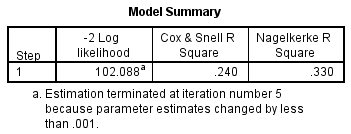
\includegraphics[width=0.9\linewidth]{images/BLogReg-Rsq}
	\caption{SPSS output}
	\label{fig:BLogReg-Rsq}
\end{figure}
\begin{itemize}
	\item Although there is no close analogous statistic in logistic regression to
	the coefficient of determination $R^2$ the Model Summary Table provides some approximations. Cox and Snell�s R-Square attempts to imitate multiple R-Square based on �likelihood�, but its maximum can be (and usually is) less than 1.0, making it difficult to interpret. 
	\item Here it is indicating that 55.2\% of the variation in the DV is explained by the
	logistic model. 
	\item Logistic regression does not have an equivalent to the R-squared that is found in OLS regression; however, many people have tried to come up with one.  
	Cox  and Snell R Square and Nagelkerke R Square - These are pseudo R-squares. 
	\item 	Nagelkerke's R-Square is a further modification of the Cox and Snell coefficient to assure that it can vary from 0 to 1. Nagelkerke's R-Square will normally be higher than the Cox and Snell measure. It is part of SPSS output and is the most-reported of the R-squared estimates.
	
	\item The Nagelkerke modification that does range from 0 to 1 is a more reliable
	measure of the relationship. Nagelkerke�s $R^2$ will normally be higher than the Cox and Snell measure.
	
	
	
	\item \textbf{Cox and Snell's R-Square} is an attempt to imitate the interpretation of multiple R-Square based on the likelihood, but its maximum can be (and usually is) less than 1.0, making it difficult to interpret. It is part of SPSS output.
\end{itemize}
%==============================================================%

\subsubsection{Nagelkerke's R-Square}
\begin{itemize}
	\item  Nagelkerke�s $R^2$ is part of SPSS output in the �Model Summary� table and is the most-reported of the R-squared estimates. 
	\item In our case it is 0.737, indicating a moderately strong relationship of 73.7\% between the predictors and the prediction.
	
	
	
\end{itemize}







\end{document}
